\section{Empirical Results}\label{sec:experiment}

In this section we present the empirical results obtained from running Hash-join, LIP and LIP-$k$ on several datasets. In Section \ref{sec:dataset}, we present the datasets we use and describe how we generate skewed and adversarial datasets. In Section \ref{sec:time} we present the running time of multiple strategies and discuss their performance. In Section \ref{sec:ratio} we discuss how $k$ affects the competitive ratio of LIP-$k$ empirically on our datasets.

\subsection{Datasets}
\label{sec:dataset}



SSB query groups 1 and 2 do not select on \texttt{DATE.YEAR} and are thus unaffected by this skew.
Query groups 3 and 4 do select on \texttt{DATE.YEAR}, so this skew can potentially affect the execution of LIP and LIP-$k$ on these queries.

\subsubsection{Skew Datasets}

We modify the normal \texttt{LINEORDER} file produced by the SSB data generator with SF = 1 to produce four skewed \texttt{LINEORDER} tables: 


\begin{itemize}
    \item \texttt{LINEORDER-DATE-50-50}: The first 50 batches have $\sigma_{\texttt{SKEW PRED}} = 1$ while the next 50 batches have $\sigma_{\texttt{SKEW PRED}} = 0$, and so on.
    In other words, The first 50 batches contain only keys satisfying \texttt{SKEW PRED}, 
    while the next 50 batches contain only keys not satisying \texttt{SKEW PRED}, 
    and so on. 

    \item \texttt{LINEORDER-DATE-FIRST-HALF}: Let $N$ be the total number of batches in \texttt{LINEORDER}. 
    The first $N/2$ batches have $\sigma_{\texttt{SKEW PRED}} = 1$ while the remaining $N/2$ batches have $\sigma_{\texttt{SKEW PRED}} = 0$.

    \item \texttt{LINEORDER-DATE-LINEAR}: $\sigma_{\texttt{SKEW PRED}}$ increases linearly from 0 to 1 across the \texttt{LINEORDER} table, 
    {\it i.e.} batch $k$ has $\sigma_{\texttt{SKEW PRED}} = k/N$.
\end{itemize}

\texttt{LINEORDER-DATE-PART-ADVERSARY}.

For simplicity in generating skew datasets, we skew the \texttt{ORDER DATE} foreign key in the \texttt{LINEORDER} table, corresponding to the primary key of the \texttt{DATE} table. 
We alter the distribution of \texttt{ORDER DATE} foreign keys satisfying \texttt{DATE.YEAR = 1997 OR DATE.YEAR = 1998}, which we will shorten to \texttt{SKEW PRED}.
Let 








Let $f_i^A$ denote the selectivity of a Bloom filter on key A after processing the $i^{th}$ batch. 
Let $\sigma_i^A$ denote the selectivity of a Bloom filter on key A on the $i^{th}$ batch alone. 






Skewed datasets are generated by first generating the SSB dataset with $\text{SF} = 1$.
We then edit the columns we want to skew. 

The aim of the adversarial dataset is to force LIP to perform the maximum number of filter probes possible, mimicking the proof of Theorem \ref{thm:det-n}.
We now show how to construct such a dataset where $n = 2$.
Let subscripts denote the batch index and superscripts denote the key column (A or B).
We start with the first batch having
$\sigma_1^A = \frac{1}{2} - \varepsilon$ and $\sigma_1^B = \frac{1}{2} + \varepsilon$ where $0 < \varepsilon < \frac{1}{2}$. Then for all $j > 1$, we let

\begin{equation*}
\sigma_j^A = 
    \begin{cases}
    1 & \text{if $j$ is even,} \\[0.5em]
    0 & \text{if $j$ is odd} \\
    \end{cases} \quad \text{and }
\sigma_j^B = 
    \begin{cases}
    0 & \text{if $j$ is even,} \\[0.5em]
    1 &  \text{if $j$ is odd}. \\
    \end{cases}
\end{equation*}

Thus, the optimal filter sequence $S^{OPT}$ is 

\begin{align*}
S^{OPT} &= 
    \begin{cases}
    (B, A) & \text{if $j$ is even}, \\[0.5em]
    (A, B) & \text{if $j$ is odd}. \\
    \end{cases}\\[0.5em]
\end{align*}

\DeclarePairedDelimiter\floor{\lfloor}{\rfloor}
After processing batch $j$,  we have $f_j^A = \frac{\frac{1}{2} - \varepsilon + \floor{\frac{j}{2}}}{j}$ and $f_j^B = \frac{\frac{1}{2} + \varepsilon + \floor{\frac{j}{2}}}{j}$  which can be rewritten as

\begin{equation*}
f_j^A = 
    \begin{cases}
    \frac{1}{2} + \frac{\frac{1}{2}-\varepsilon}{j} & \text{if $j$ is even}, \\[0.5em]
    \frac{1}{2} - \frac{\varepsilon}{j} &  \text{if $j$ is odd}; \\
    \end{cases}  \quad \text{and }
f_j^B = 
    \begin{cases}
    \frac{1}{2} - \frac{\frac{1}{2}-\varepsilon}{j} & \text{if $j$ is even}, \\[0.5em]
    \frac{1}{2} + \frac{\varepsilon}{j} &  \text{if $j$ is odd}, \\
    \end{cases}\\[0.5em]
\end{equation*}

and thus, LIP's filter ordering will be

\begin{align*}
S &= 
    \begin{cases}
    (A, B) & \text{if $j$ is even}, \\[0.5em]
    (B, A) & \text{if $j$ is odd}, \\
    \end{cases}\\[0.5em]
\end{align*}

which is the reverse of $S^{OPT}$. 
Hence, after the first batch has been processed, LIP will have worst-case performance on all remaining batches.


We summarize the skew datasets studied in this paper in Table~\ref{tab:skew_datasets}

\begin{center}
\begin{tabular}{ |>{\ttfamily}r|>{\ttfamily}c|l| } 
\hline
{\bf Dataset Name} & {\bf Skewed Foreign Keys} & {\bf Description of Skew} \\
\hline
\hline
lineorder-date-50-50& ORDER DATE & First 50 batches have $\sigma_{\texttt{SKEW PRED}} = 1$ \\
& & Next 50 batches have $\sigma_{\texttt{SKEW PRED}} = 0$ \\ 
\hline
lineorder-date-first-half& ORDER DATE & First $N/2$ batches have $\sigma_{\texttt{SKEW PRED}} = 1$ \\
& & Next $N/2$ batches have $\sigma_{\texttt{SKEW PRED}} = 0$, \\
& & where $N$ is the total number of batches in \text{LINEORDER}\\
\hline
lineorder-date-linear& ORDER DATE & $\sigma_{\texttt{SKEW PRED}}$ increases linearly from 0 to 1 \\
\hline
lineorder-date-part-adversary& ORDER DATE & See Section~\ref{sec:ratio}\\
\hline
\end{tabular}
\end{center}

The adversarial dataset is constructed to make SSB query 4.2 achieve near worst-case performance for LIP. 



\subsection{Execution Time}
\label{sec:time}



\subsection{Competitive Ratio}
\label{sec:ratio}

We ran LIP-$k$ on each skewed dataset we produced and compute the competitive ratio of each LIP-$k$ by taking the maximum of the competitive ratios achieved across all queries in all datasets. The results are depicted in Figure \ref{fig:cr}. 

\begin{figure}
    \centering
    \subfloat[]{
        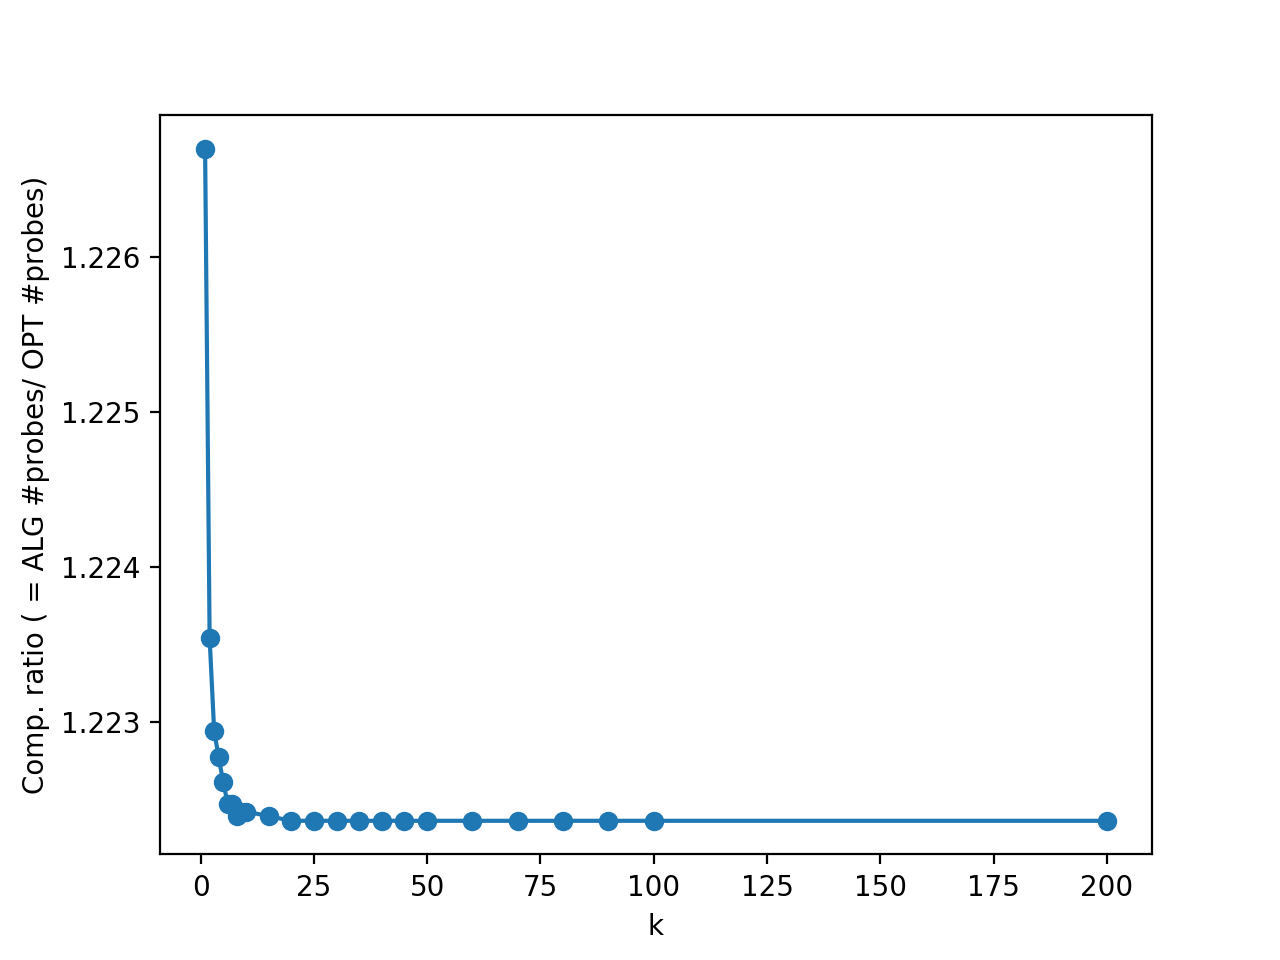
\includegraphics[width=0.43\textwidth,keepaspectratio]{cr-k-uniform}
    }   
    \quad
    \subfloat[]{
        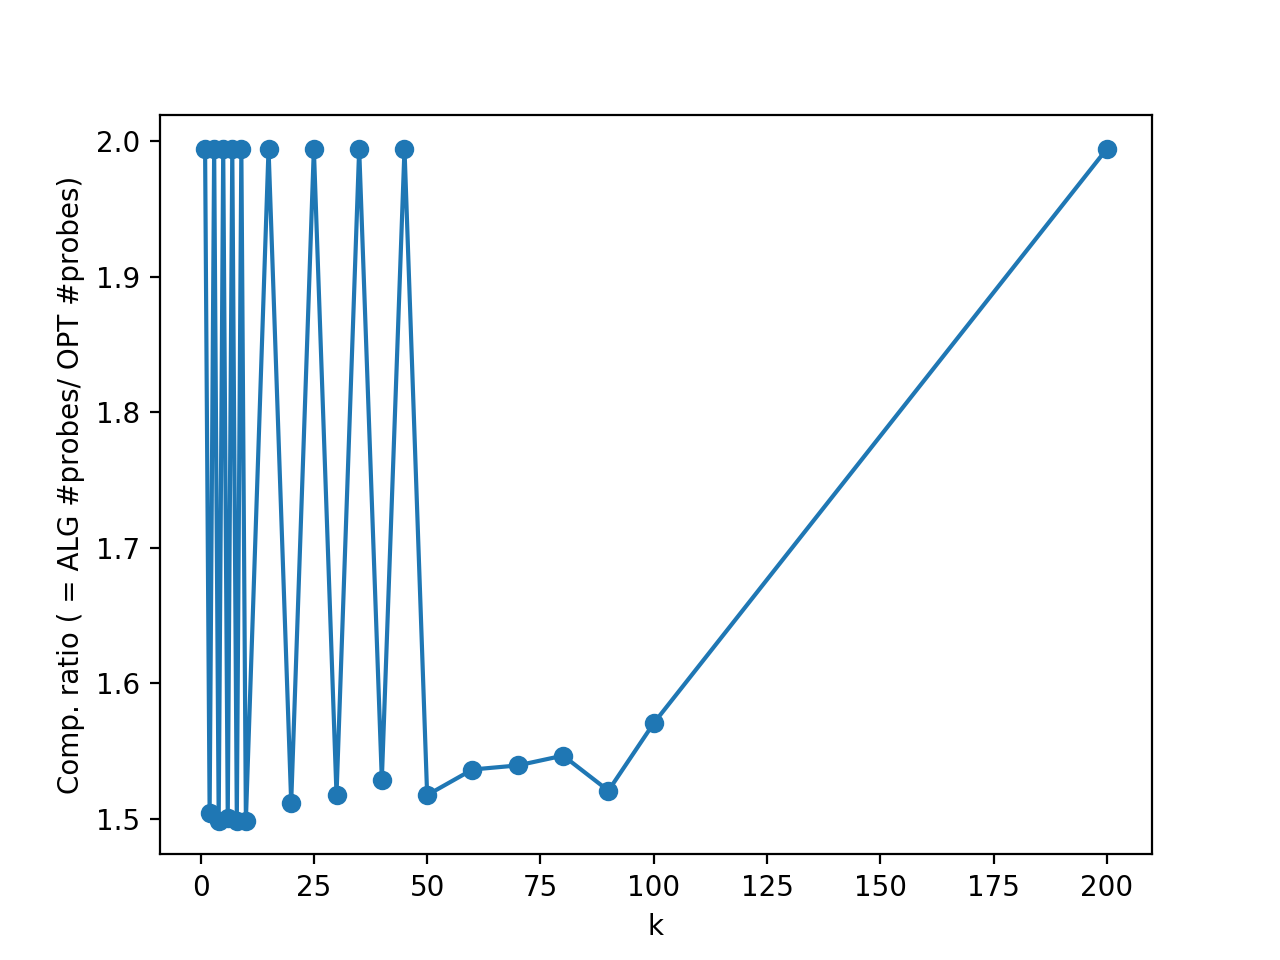
\includegraphics[height=0.32\textwidth,keepaspectratio]{cr-k-skewed}
    }
    \caption{The competitive ratios of LIP-$k$ against different $k$ values. We ran LIP-$k$ on uniform data and skewed (and adversarial) dataset to produce (a) and (b) respectively. The data point at $k = 200$ represents LIP (which is essentially LIP-$\infty$).}
    \label{fig:cr}
\end{figure}

When the keys in the fact table columns are distributed uniformly, the filters need not react to the local changes. Hence for LIP with higher $k$, it remembers more batches in the uniform data, therefore may produce relatively more accurate estimate of the selectivities than the LIP with lower $k$. Hence the competitive ratio would decrease (slightly) when $k$ increases, as depicted in Figure \ref{fig:cr}.  

%@TODO: Explain the adversarial case using epsilons
Figure \ref{fig:cr} (b) displays how an adversarial dataset can make LIP-$k$ and LIP perform inefficiently. In fact, each LIP-$k$ with even $k$ achieves an approximation ratio less than 2; LIP and LIP-$k$ with odd $k$ achieve an approximation ratio of almost 2 precisely at Query 3.2 in dataset \texttt{date-part-adversary}. Query 3.2 has two joins, and thus the performance of LIP-$k$ with even $k$ matches the worst case competitive ratio. By construction of \texttt{date-part-adversary}, the first batch has $\sigma^{1}_{1} = 1/2-\
\varepsilon$ and $\sigma^{1}_{2} = 1/2+\varepsilon$, and  each batch $B_{2i+1}$ is an \textit{odd} batch, with $\sigma^{2i}_{1} = 0$ and $\sigma^{2i}_{2} = 1$; and each batch $B_{2i}$ is an \textit{even} batch, with $\sigma^{2i}_{1} = 1$ and $\sigma^{2i}_{2} = 0$. 

When $i \leq k$, LIP and LIP-$k$ execute identically, since LIP-$k$ has not yet ``forgotten" any previous batches. We now consider the case where $i > k$, {\it i.e.} where LIP-$k$ has forgotten at least the first batch. For odd $k$, LIP-$k$'s selectivity estimates always contains one more odd (or even) batch than the other, and thus the estimated selectivity and filtering sequence are in favor of the majority batch type. This yields a false prediction of the next batch, yielding a competitive ratio of 2. For even $k$, LIP-$k$'s selectivity estimates contain an equal amount of even an odd batches,  and thus estimated selectivities remain the same ($1/2$ by construction) throughout the execution, and the filter sequence does not change. Thus for half batches it is optimal, and for the other half it is worse, resulting in a competitive ratio of \[ \frac{1 \times 1/2 + 2 \times 1/2}{1} = 1.5,\] as depicted in Figure \ref{fig:cr}. For LIP, since it remembers the statistics from the beginning, by construction it would also make the same decision as LIP-$k$ with odd $k$, losing at every batch. 

LIP performs poorly because it never forgets the first batch.
%@TODO: I will explain this better!!!!
\footnote{An astute observer might notice that for $k = 200$, the worst-case competitive ratio of $2$ is achieved even though $k$ is not odd. This is explained by recognizing that LIP-200 is essentially an approximation of LIP. LIP-200 performs just as poorly as LIP up until  the $201^{st}$ batch, after which it estimates both selectivities as 1/2.}



\begin{align*}
\varepsilon_i = 
    \begin{cases}
    \frac{\varepsilon}{2k+1} & \text{for odd $i$, where $i = 2k + 1$} \\ 
    \frac{\frac{1}{2} - \varepsilon}{2k} & \text{for even $i$, where $i = 2k$}
    \end{cases}
\end{align*}

If $k$ is even, then LIP-k will (after the first $k$ batches have been processed) have $\sigma^A_i = \sigma^B_i = \frac{1}{2}$. Thus,

%$k = 1, 2, 3, 4, 5, 10, 15, 20, 25, 30, 35, 40, 45, 50, 60, 70, 80, 90, 100$ on 